\chapter{Anvendelsesgrænsetilstand}
Nu er brudgrænsetilstanden bestemt, i det følgende regnes anvendelsesgrænsetilstanden. Ud fra anvendelsesgrænsetilstanden kan det vurderes, om bygningen har tilstrækkelig små deformationer til, at bygningens dimensioner kan godtages. 
\newline \indent{     }  Det antages, at der kun virker én variabel last på konstruktionen, nemlig vindlasten. Denne last forlænges helt ned til understøtningerne, og der ses bort fra jordlasten. Derfor er der udregnet nye reaktioner for konstruktionen, som ses i Tabel \ref{tab:anden}. Beregningerne kan ses i Bilag XX. 

\begin{table}
	\begin{center}
		\begin{tabular}{|c|c|c|}
			\hline
			Reaktion & Værdi & Enhed \\ \hline
			$S_x$ & -71,14 		& kN      \\ \hline
			$C_y$ & 578,86 		& kN      \\ \hline
			$S_y$ & 36,07 		& kN       \\ \hline
			$B_y$ & 1432,31 	& kN      \\ \hline
			$A_y$ & 344,53 		& kN      \\ \hline
			$B_x$ & 0,00 		& kN      \\ \hline
			$A_x$ & -147,87 	& kN       \\ \hline
		\end{tabular}
		\caption{Reaktioner for anvendelsesgrænsetilstand}
		\label{tab:anden}
	\end{center}
\end{table}

\section{Moment}
Der er lavet i alt fem snit på konstruktionen, som vist på Figur \ref{fig:snitanvendelse}. Dog ses der bort fra den højre del af konstruktionen, og dermed er det kun snit 1-3 der anvendes. 

\begin{figure}[H]
	\centering
	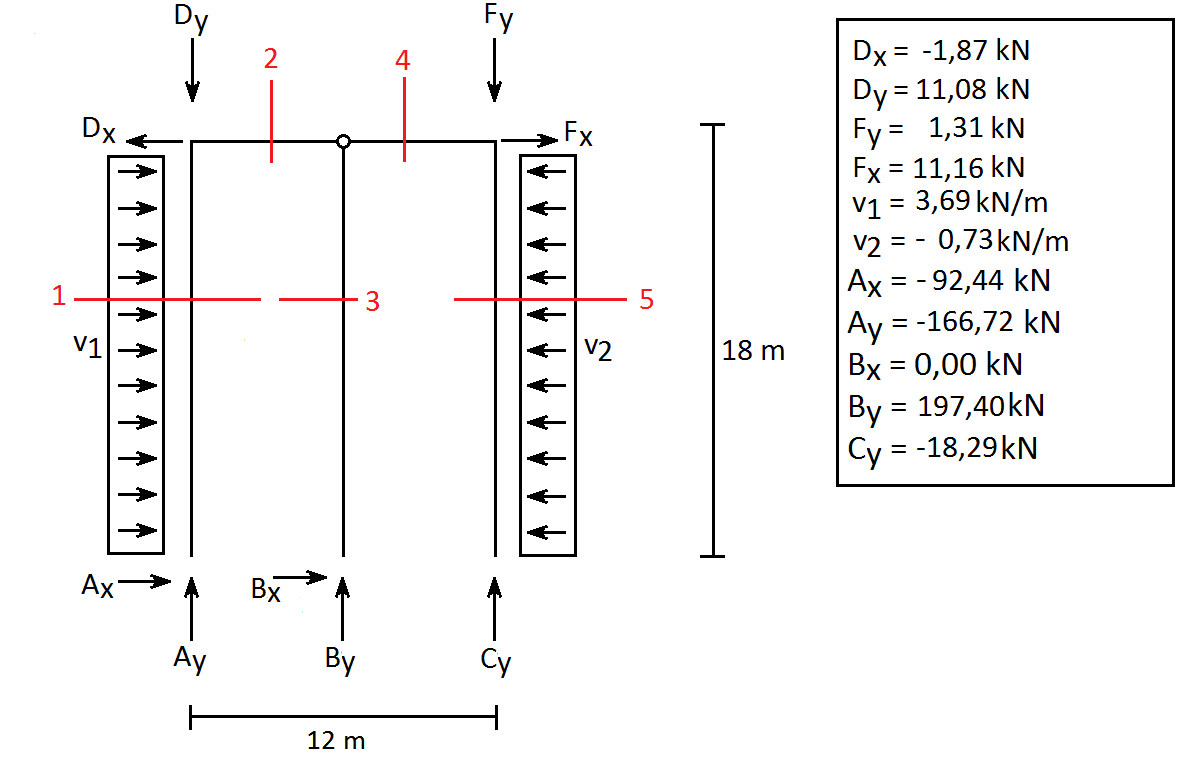
\includegraphics[width=0.9\textwidth]{billeder/snitanvendelse.png}
	\caption{Snit}
	\label{fig:snitanvendelse}
\end{figure}

Nedenfor er vist et eksempel på, hvordan momentligningen regnes for snit 1. Alle beregningerne findes i Bilag XX.
\newline
\newline
\textbf{Snit 1: 0 m < x < 18 m}
\newline
Fritlegemediagrammet for snit 1 ses på Figur \ref{fig:snitetan}.
\begin{figure}[H]
	\centering
	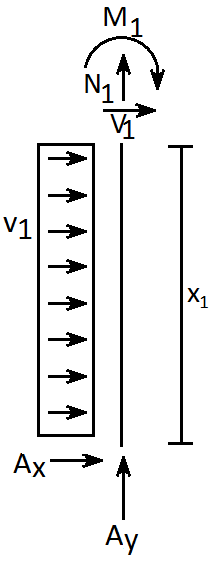
\includegraphics[width=0.2\textwidth]{billeder/asnitet.png}
	\caption{Snit 1}
	\label{fig:snitetan}
\end{figure}


Først bestemmes momentligningen for snit 1, 2 og 3 disse kaldes for $M_1$, $M_2$ og $M_3$:
\begin{center}
	$0 = M_1 + A_x \cdot x + Vind_1\cdot x\cdot \frac{x}{2} \leftrightarrow M_1(x) = A_x\cdot x_1 -\frac{1}{2}\cdot Vind_1 \cdot x_1^2$
\end{center}

\begin{center}
	$0 = M_1 + A_x \cdot x + Vind_1\cdot x\cdot \frac{x}{2} \leftrightarrow M_1(x) = A_x\cdot x_1 -\frac{1}{2}\cdot Vind_1 \cdot x_1^2$
\end{center}

\begin{center}
	$0 = M_1 + A_x \cdot x + Vind_1\cdot x\cdot \frac{x}{2} \leftrightarrow M_1(x) = A_x\cdot x_1 -\frac{1}{2}\cdot Vind_1 \cdot x_1^2$
\end{center}

\section{Bjælkens differentialligning}
For at udregne udbøjningerne for stængerne, anvendes bjælkens differentialligning. Da det statiske system for tilbygningen til Strøybergs Palæ er statisk bestemt, er det den anden ordens afledede, som anvendes for at bestemme udbøjningerne.
\newline
<<<<<<< HEAD
Først findes den første og anden aflede for $M_1$: 
=======
Først findes den første og anden aflede for $M_1$: %Her vises integration%
>>>>>>> origin/master
 
\begin{equation}
	$\int M_1(x_1) = \int \frac{- A_x\cdot x_1 - \frac{1}{2}\cdot V_1 \cdot x_1^2$}{EI}
	= \alpha_1(x_1) = \int \frac{-\frac{1}{2} A_x x_1^2 - \frac{1}{6}  V_1  x_1^3 }{EI}
\end{equation}

\begin{equation}
	$\int \alpha_1(x_1) = \int \frac{-\frac{1}{2} A_x x_1^2 - \frac{1}{6}  V_1  x_1^3 }{EI}
	= u_1(x_1) = \int \frac{{1}{6} A_x x_1^3 - \frac{1}{24}  V_1  x_1^4 }{EI} + k_1 x_1 + k_2$
\end{equation}

Samme metode bruges på de næste 2 momentligninger og det giver følgende udgangspunkt: 
\newline
$M_2$:
\begin{center}
	$M_2(x_2) = M_1 + A_x \cdot x + Vind_1\cdot x\cdot \frac{x}{2} \leftrightarrow M_1(x) = A_x\cdot x_1 -\frac{1}{2}\cdot Vind_1 \cdot x_1^2$
\end{center}

\begin{center}
	$M_2(x_2) = M_1 + A_x \cdot x + Vind_1\cdot x\cdot \frac{x}{2} \leftrightarrow M_1(x) = A_x\cdot x_1 -\frac{1}{2}\cdot Vind_1 \cdot x_1^2$
\end{center}

\begin{center}
	$M_2(x_2) = M_1 + A_x \cdot x + Vind_1\cdot x\cdot \frac{x}{2} \leftrightarrow M_1(x) = A_x\cdot x_1 -\frac{1}{2}\cdot Vind_1 \cdot x_1^2$
\end{center}

<<<<<<< HEAD
$M_3$ 
=======
$M_3$: 
>>>>>>> origin/master

\begin{center}
	$M_2(x_2) = M_1 + A_x \cdot x + Vind_1\cdot x\cdot \frac{x}{2} \leftrightarrow M_1(x) = A_x\cdot x_1 -\frac{1}{2}\cdot Vind_1 \cdot x_1^2$
\end{center}

\begin{center}
	$M_2(x_2) = M_1 + A_x \cdot x + Vind_1\cdot x\cdot \frac{x}{2} \leftrightarrow M_1(x) = A_x\cdot x_1 -\frac{1}{2}\cdot Vind_1 \cdot x_1^2$
\end{center}

\begin{center}
	$M_2(x_2) = M_1 + A_x \cdot x + Vind_1\cdot x\cdot \frac{x}{2} \leftrightarrow M_1(x) = A_x\cdot x_1 -\frac{1}{2}\cdot Vind_1 \cdot x_1^2$
\end{center}

Ved integrering af ligningningerne giver dette 6 ligningner med 6 ubekænkte konstanter. Dette kan løses ved at opstille 6 randbetingelser som er: 

%tabel med randbetingelser%

De opsatte randbetingelser regnes ud og følgende 6 konstanter får værdierne: 

%Tabel med konstant værdierne% 

<<<<<<< HEAD
Konstanterne for den anden aflede af $M_1$ indsættes i ligningen og kurven udregnes. Dernæst findes den maksimale udbøjning, det gøres også for $M_2$ og $M_3$ og følgende 3 maksimale udbøjninger fåes: 
=======
Konstanterne for den anden aflede af $M_1$ indsættes i ligningen og kurven udregnes. Dernæst findes den maksimale udbøjning, det gøres også for den anden aflede af $M_2$ og $M_3$ og følgende 3 maksimale udbøjninger fåes: 
>>>>>>> origin/master

%tabel for udbøjninger% 

Konklusion